\documentclass[conference]{IEEEtran}

% *** GRAPHICS RELATED PACKAGES ***
%
\ifCLASSINFOpdf
  \usepackage{graphicx}
  % declare the path(s) where your graphic files are
  \graphicspath{{./figures/}}
  \DeclareGraphicsExtensions{.pdf,.jpeg,.png,.jpg}
\else
  \usepackage{graphicx}
  % declare the path(s) where your graphic files are
  \graphicspath{{./figures/}}
  \DeclareGraphicsExtensions{.eps}
\fi

\usepackage{multirow}
\usepackage{float}


\begin{document}
% paper title
% can use linebreaks \\ within to get better formatting as desired
% Do not put math or special symbols in the title.
\title{On Clustering Stocks Using Granger Causality}

% author names and affiliations
\author{
\IEEEauthorblockN{Richard Al-Bayaty}
\IEEEauthorblockA{School of Electrical and Computer Engineering\\
University of Florida\\
Gainesville, FL 32611\\
Email: ralbayaty@ufl.edu}
\\
}

\maketitle


\begin{abstract}
%Abstract - A paragraph that summarizes the problem and the results.
When analyzing the stock market for trading, it is conducive to consider relationships between stocks in order to best make decisions regarding buying and selling. If one were to have an exact causal relationship between stocks, it would be possible to accurately make predictions based on the movement of one stock, given the history of movements of both stocks and the causal relationship to the other. A crude mechanism for modeling this causation is to utilize Granger causality. The premise behind this causality construction is that one variable Granger causes another if knowing the joint information of the variables' history provides more information for prediction than knowing just the single variables' history.

 
\end{abstract}
\hfill

\begin{IEEEkeywords}
Clustering, financial time series, Granger causality, S\&P500.
\end{IEEEkeywords}

\section{Introduction}
%	Introduction - Sets the context, describes the problem, and describes your solution.
When examining multivariate time series data, several assumptions are often made to help simplify the problem at hand. Firstly, stationarity is often assumed to allow a time series to be examined over a time interval without the need to be concerned with means and variances changing as a function of time. Another assumption is that there exists an underlying relationship between the variables which is slow to change over time, especially in comparison to the faster variation in the time signal of the variables themselves. Another assumption for the data is that a vector autoregressive (VAR) model can be fit to it. What this means is that at each time step a variable can be constructed as a linear combination of its previous values. Using these three assumptions, the multivariate time series that is the US stock market could potentially be modeled in such a way as to capture both the causal relationship of the variables and the variable affinities to congregate or separate from each other. The task at hand is to determine if a causal structure can help to identify an applicable means of clustering stocks utilizing their time series stock price data and the Granger causality of that multivariate data.

% Paper organization: Section I, Section II, etc...
The rest of the study is organized as follows: Section II covers the work related to this project and gives an overview of some of the currently used for stock clustering, Section III covers the methodology and analysis techniques, Section IV discusses the experiments performed using the algorithms described in Section III and shows visualizations of algorithm outputs, and lastly, Section V concludes the study with a summary and future work.

\section{Related Work}
%	Related work - Describes representative works related to your work, and summarizes the pros and cons of each work.
Since the presumption that the multivariate stock data contains stationary variables, which is an inherently risky assumption in the first place, published works regarding clustering of stocks have a different handling. Other models of causality are often used as well, instead of the common Granger causality.

 Foresti tested for Granger Causality between stock prices and economic growth and found that the relationship found was unidirectional. The stock prices could be used to predict economic growth, the the economic growth was not capable of predicting stock prices, in his framework \cite{Foresti}.
 
 Hendahewa and Pavlovic used machine learning techniques to help learn the coefficients of a modified auto regressive conditional heteroskedasticity model \cite{Henda}. This model was used to analyze fluctuations in volatility over various economic conditions and assisted in uncovering correlations in external factors to the data. Their proposed model was a sparse linear regression model with a smoothness constraint. The authors used Dynamic Time Warping to make comparable length external factor time sequences which matched the stock data better.
 
 Isogai uses a similar model as Hendahewa and Pavlovic to perform clustering of Japanese stock returns, except that Isogai uses a novel technique to make automated cluster sizes from a correlation matrix of standardized returns using a recursive spectral clustering with modularity optimization. Adding further merit to the work, he performs random portfolio simulations to help show that his technique aides in portfolio risk management.



\section{Description}
%	Description - One or more sections that describes the problem and your approach to the solution in detail.
\subsection{Granger Causality}
The concept of Granger causality was developed by none other than C.W.J. Granger himself \cite{Granger}. In the multivariate case, a variable is said to Granger cause another when the following applies:
$$ \sigma^2(X|\overline{U}) < \sigma^2(X|\overline{U-Y}),$$
 that is to say that the universe of information U provides less variance than the universe of information available without the variable Y. This can be extended further to incorporate a sense of time lag of causation by allowing for a time lag, k, after showing a causation in the sense shown earlier by the following:
$$ \sigma^2(X|U-Y(k)) < \sigma^2(X|U-Y(k+1)),$$ 
which signifies that knowing information about Y at time steps prior to k does not increase predictability of X. 

\subsection{Dataset}
The data used in this project consists of the 502 stock tickers of the S\&P500. The 28 work-day period between 11/01/2014 to 12/11/2014 was used to construct a data matrix of size 502x28. The MATLAB builtin connection to Yahoo! Finance is used to collect the data. While reliability of the data is important in most cases, the use of this dataset for clustering can afford potential rounding or minor calculation errors (of significance less than a cent) induced by the Yahoo! accumulation and processing of the data.

\subsection{Methods}
After gathering the stock data, a pairwise Granger causality is calculated with a fixed time lag of 5 days and significance level of 0.01. The time lag represents how many previous time steps behind to incorporate into the multivariate VAR model. The significance level is the level at which you want the F-test to be higher than to reject the null hypothesis that the second variable does not Granger caused by the first. A new matrix is constructed in order to give a measure of ``distance'' to the distance matrix. This new matrix is made entry-wise by taking the F-test score from the Granger causality function and dividing it by the critical value for the F-test on the data at the provided significance level, $$G_{soft} = \frac{F}{value_{critical}} $$ where F is the F-test score and $value_{critical}$ is the critical value for the F-test to pass. This method allows for values according to the following:
$G_{soft} \geq 1 $, when Granger causality exists, and $ G_{soft} < 1$, when there is no reported causality.

Clustering is performed using three methods: Unnormalized Spectral Clustering, Normalized Spectral Clustering (Ng, Jordan, and Weiss), and Normalized Spectral Clustering (Shi and Malik) \cite{Luxburg}. For a high level analysis, the clustering methods are considered to have been successful if the distribution of the labels for the clusters is similar to the true distribution of labels for the stock. The true labels are considered to be the S\&P500 Sector labels given to each stock. These algorithms require that the number of clusters be passed as a parameter, so the true number of clusters is used. After the clustering, the new labels are compared with the true labels and if there is both a similarity in the distribution of the labels and a high occurrence of specific pairs of labels, then the algorithm is said to have closely reciprocated the true labels from the Granger Causality matrix. The reason for using pairs of occurrences of labels is that if all of one type of sector was labeled as being ``A'' in truth and got labeled ``B'' as output from the algorithm, then the actual numbering of the labels is irrelevant since the stocks are being clustered based on similarity of sector, and the groupings ultimately were the same.

The MATLAB ``Granger Causality Test'' function was used from Chandler Lutz to implement the generation of the Granger Causality matrix.



\section{Evaluation}
%	Evaluation - A section that quantitatively evaluates your ideas.
The proposed method yielded various results for the clustering of the stocks into 10 groups to simulate the 10 sectors of the S\&P500. Each of the three different spectral clustering techniques used offered a different grouping of stocks. Since the clustering labels overlapped in various ways with the original labels, a maximizing of occurrence approach was taken to make hard thresholding of the label possible for the mismatching stocks. This approach was performed by making a matrix consisting of an occurrence count at the $(i,j)$ component corresponding to the $i^{th}$ label (the truth) pairing with the $j^{th}$ label (the output of the clustering algorithm). The results of this can be seen in Tables \ref{tab:pairing1}, \ref{tab:pairing2}, and \ref{tab:pairing3}. The clustering techniques used are respectively the same as discussed earlier.



\begin{table}[h]
\renewcommand{\arraystretch}{1.2}
\caption{Label pairings after clustering using $L$} \label{tab:pairing1}
\centering
\begin{tabular}{c||cccccccccc}
& 1 & 2 & 3 & 4 & 5 & 6 & 7 & 8 & 9 & 10\\
\hline \hline
1 & 0 & 1 & 0 & 1 & 0 & 80 & 1 & 0 & 0 & 1\\ 
2 & 1 & 0 & 0 & 0 & 0 & 38 & 0 & 1 & 0 & 0\\ 
3 & 0 & 0 & 0 & 0 & 0 & 42 & 0 & 2 & 0 & 0\\ 
4 & 0 & 0 & 0 & 0 & 0 & 83 & 0 & 3 & 0 & 0\\ 
5 & 0 & 0 & 0 & 0 & 2 & 52 & 0 & 1 & 0 & 0\\ 
6 & 0 & 0 & 0 & 0 & 0 & 66 & 0 & 0 & 0 & 0\\ 
7 & 0 & 0 & 0 & 0 & 0 & 61 & 0 & 1 & 0 & 0\\ 
8 & 0 & 0 & 0 & 0 & 0 & 28 & 0 & 1 & 0 & 0\\ 
9 & 1 & 0 & 0 & 0 & 0 & 5 & 0 & 0 & 0 & 0\\ 
10 & 1 & 0 & 1 & 0 & 3 & 24 & 0 & 0 & 1 & 0 
\end{tabular}
\end{table}

\begin{table}[h]
\renewcommand{\arraystretch}{1.2}
\caption{Label pairings after clustering using $L_{sym}$} \label{tab:pairing2}
\centering
\begin{tabular}{c||cccccccccc}
& 1 & 2 & 3 & 4 & 5 & 6 & 7 & 8 & 9 & 10\\
\hline \hline
1 & 6 & 8 & 7 & 10 & 9 & 12 & 3 & 10 & 9 & 10\\ 
2 & 7 & 6 & 1 & 1 & 7 & 2 & 1 & 2 & 3 & 10\\ 
3 & 4 & 4 & 6 & 2 & 14 & 2 & 1 & 4 & 6 & 1\\ 
4 & 10 & 9 & 6 & 5 & 12 & 8 & 2 & 6 & 19 & 9\\ 
5 & 6 & 1 & 5 & 4 & 6 & 3 & 4 & 11 & 4 & 11\\ 
6 & 7 & 5 & 13 & 6 & 9 & 3 & 4 & 8 & 8 & 3\\ 
7 & 7 & 4 & 2 & 8 & 10 & 1 & 5 & 9 & 7 & 9\\ 
8 & 3 & 3 & 3 & 1 & 2 & 6 & 2 & 3 & 4 & 2\\ 
9 & 0 & 1 & 0 & 1 & 1 & 0 & 0 & 2 & 0 & 1\\ 
10 & 1 & 8 & 0 & 2 & 5 & 0 & 1 & 7 & 3 & 3 
\end{tabular}
\end{table}


\begin{table}[h]
\renewcommand{\arraystretch}{1.2}
\caption{Label pairings after clustering using $L_{rw}$} \label{tab:pairing3}
\centering
\begin{tabular}{c||cccccccccc}
& 1 & 2 & 3 & 4 & 5 & 6 & 7 & 8 & 9 & 10\\
\hline \hline
1 & 5 & 6 & 17 & 3 & 10 & 13 & 24 & 1 & 0 & 5\\ 
2 & 2 & 3 & 7 & 4 & 10 & 4 & 7 & 1 & 0 & 2\\ 
3 & 2 & 5 & 4 & 5 & 4 & 8 & 12 & 2 & 0 & 2\\ 
4 & 8 & 1 & 11 & 22 & 19 & 6 & 10 & 4 & 0 & 5\\ 
5 & 4 & 2 & 12 & 5 & 15 & 4 & 5 & 1 & 1 & 6\\ 
6 & 6 & 4 & 10 & 7 & 9 & 9 & 13 & 4 & 0 & 4\\ 
7 & 4 & 2 & 7 & 4 & 14 & 11 & 13 & 2 & 0 & 5\\ 
8 & 5 & 1 & 4 & 6 & 4 & 3 & 4 & 2 & 0 & 0\\ 
9 & 0 & 0 & 0 & 0 & 0 & 1 & 5 & 0 & 0 & 0\\ 
10 & 2 & 8 & 0 & 6 & 5 & 3 & 5 & 0 & 0 & 1 
\end{tabular}
\end{table}


The output of the hard thresholding step, which was done by using the pairing with maximum number of occurrences, is shown in Table \ref{tab:maxpair}. In total for each algorithm there were 1, 7, and 4, unique pairings after thresholding. This shows that using the unnormalized clustering algorithm is not beneficial, while the normalized versions have potential to make meaningful groupings of the stocks, potentially for predictability purposes.

\begin{table}[h]
\renewcommand{\arraystretch}{1.2}
\caption{Label pairings after maximizing} \label{tab:maxpair}
\centering
\begin{tabular}{c||ccc}
& $L$ & $L_{sym}$ & $L_{rw}$ \\
\hline \hline
1 & 6 & 6 & 7 \\ 
2 & 6 & 10 & 5 \\ 
3 & 6 & 5 & 7\\ 
4 & 6 & 9 & 4 \\ 
5 & 6 & 8 & 5 \\ 
6 & 6 & 3 & 7 \\ 
7 & 6 & 5 & 5\\ 
8 & 6 & 6 & 4\\ 
9 & 6 & 8 & 7\\ 
10 & 6 & 2 & 2 
\end{tabular}
\end{table}



\begin{figure}[H] 
\begin{center}
  \noindent
  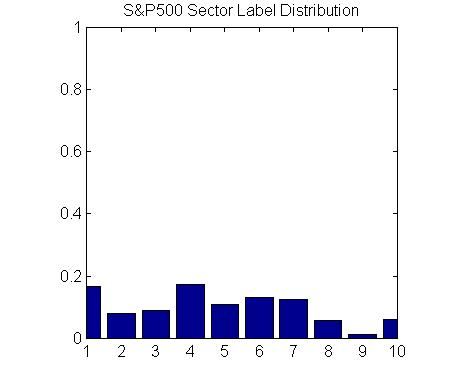
\includegraphics[width=.4\columnwidth]{original_distro}
  \caption{The original distribution of the labels}  \label{fig:original}
\noindent
  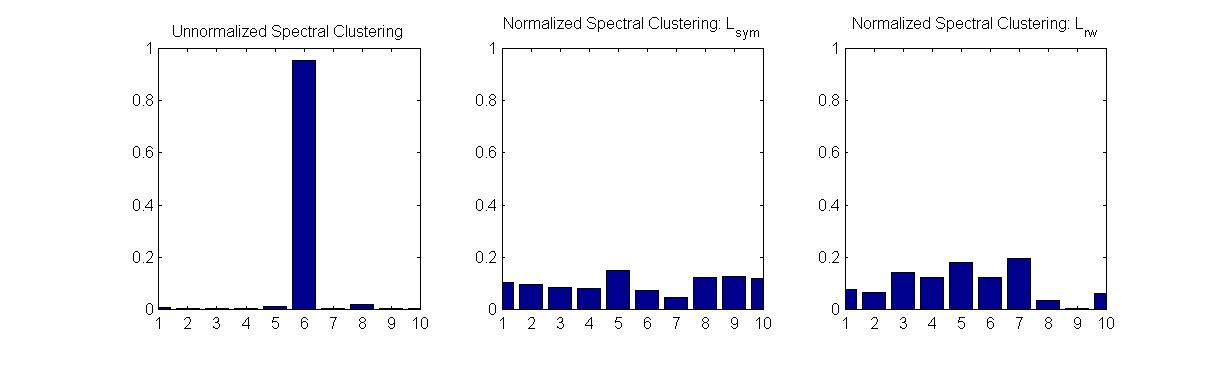
\includegraphics[width=\columnwidth]{distros} 
  \caption{The distribution of labels from spectral clustering} \label{fig:distro}
\end{center}
\end{figure}

The distribution of labels are shown in Figures \ref{fig:original} and \ref{fig:distro}. The labels are bunched into a few small groups and one large group in the unnormalized spectral clustering, while the normalized spectral clustering algorithms offered a more diverse and similar representation as the true labels.

\section{Conclusion}
%	Summary and Conclusions - Summarize what you did and what interesting things you learned from the project.
Granger causality was considered as a method of constructing a distance matrix for use in common spectral clustering algorithms. While the outputs differed visibly, the results could very well be an appropriate means of grouping the stocks in various ways for purposes such as risk management or variable risk/reward investment strategies. Other methods of making variable level clusterings could be implemented in future works, since a hard thresholding method was used in this work and decimated the underlying hierarchical structure discovered by the various spectral clustering algorithms. Other forms of clustering, such as using modularity maximization could also be utilized to better implement this algorithm for applicable tasks in future work. A more extensive dataset would be used for future work as well, as cyclic tendencies could be captured as well such as seasonal trends.



% references section

% can use a bibliography generated by BibTeX as a .bbl file
% BibTeX documentation can be easily obtained at:
% http://www.ctan.org/tex-archive/biblio/bibtex/contrib/doc/
% The IEEEtran BibTeX style support page is at:
% http://www.michaelshell.org/tex/ieeetran/bibtex/
%\bibliographystyle{IEEEtran}
% argument is your BibTeX string definitions and bibliography database(s)
%\bibliography{IEEEabrv,../bib/paper}
%
% <OR> manually copy in the resultant .bbl file
% set second argument of \begin to the number of references
% (used to reserve space for the reference number labels box)
\begin{thebibliography}{7}


\bibitem{Foresti}
Foresti, Pasquale. "Testing for Granger causality between stock prices and economic growth." (2006). url:http://mpra.ub.uni-muenchen.de/2962/

\bibitem{Henda}
Hendahewa, Chathra, and Vladimir Pavlovic. "Analysis of Causality in Stock Market Data." In Machine Learning and Applications (ICMLA), 2012 11th International Conference on, vol. 1, pp. 288-293. IEEE, 2012.

\bibitem{Isogai}
Isogai, Takashi. "Clustering of Japanese stock returns by recursive modularity optimization for efficient portfolio diversification." Journal of Complex Networks 2, no. 4 (2014): 557-584.


\bibitem{Granger}
Granger, Clive WJ. "Investigating causal relations by econometric models and cross-spectral methods." Econometrica: Journal of the Econometric Society (1969): 424-438.


\bibitem{Luxburg}
Von Luxburg, Ulrike. "A tutorial on spectral clustering." Statistics and computing 17, no. 4 (2007): 395-416.

\bibitem{Cause}
Lutz, Chandler. ``Granger Causality Test.'' url: http://kr.mathworks.com/matlabcentral/fileexchange/25467-granger-causality-test/content/granger\_cause.m


\end{thebibliography}




\end{document}